 % !tex root= main.tex
\section{Formation de la synapse}
	\label{sec:IntroSynapse}
	La \gls{jnm} est une synapse appartenant au \gls{snp}, qui permet la transmission nerveuse entre le motoneurone et la fibre musculaire squelettique. La \gls{jnm} est indispensable à la survie en permettant les mouvements volontaires et la respiration. De part sa grande taille et sa facilité d'accès, la \gls{jnm} est depuis longtemps le modèle préférentiel d'étude des synapses du point de vue structural, développemental, et physiologique. Chez les vertébrés, le neurotransmetteur utilisé à la \gls{jnm} est l'\gls{ach}. 
	
	L'apposition de l'élément pré-synaptique sur l'élément post-synaptique requiert au préalable une différenciation post-synaptique qui e manifeste par la présence d'agrégats de \glspl{achr} au milieu de la fibre musculaire, agrégats qui commencent à se former avant l'arrivée de l'axone \cite{Wu2010a, Gordon2012}. Cette étape qui se déroule avant la reconnaissance et l'ancrage de l'axone sur l'élément post-synaptique, et se se nomme "pré-patterning". Elle dépend entièrement de la présence de \acrshort{musk}, un récepteur tyrosine kinase qui va donc avoir plusieurs rôles dans la formation de la \gls{jnm} : attirer l'axone, stimuler et remodeler les agrégats de \gls{achr} chez l'embryon et maintenir la synapse chez l'adulte.
	
	Lors du développement, le cône de croissance de l'axone se dirige vers l'élément post-synaptique (voir \cref{fig:FormaJNM}). Quand les deux éléments entrent en contacts (au jour embryonnaire E14 chez la souris), des cascades de signalisation sont initiées, ce qui résulte en la différentiation des partie pré- et post-synaptiques \cite{Sanes1999}, avec notamment une redistribution des clusters de \glspl{achr}, qui ne sont plus présent dans les régions extrasynaptiques.
	
	\begin{figure}[h]
		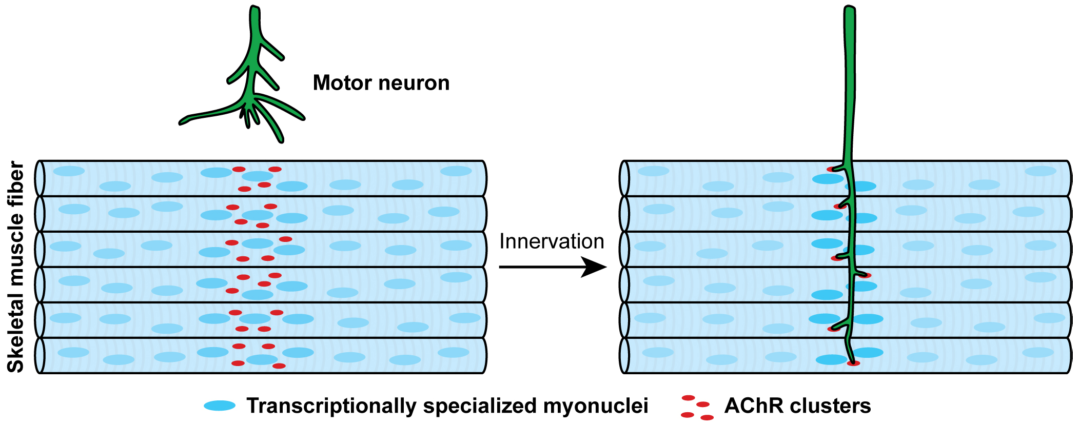
\includegraphics[width=\textwidth]{./Images/formation_jnm.png}
		\caption{Formation de la \gls{jnm}.} 
		\descfig{Figure issue de Burden \emph{et al.} 2018 \cite{Burden2018}.}
		\label{fig:FormaJNM}
	\end{figure}
	
	Cette accumulation de \glspl{achr}, comme d'un certain nombre de protéines synaptiques, est due à un récepteur particulier : \gls{musk}. Ce dernier joue un rôle clef dans la formation de la synapse, sa position déterminant la position de cette dernière \cite{DeChiara1996, Glass1996}. Le ligand activateur de \gls{musk} est historiquement l'Agrine \cite{Glass1996}, qui est sécrété par l'axone au contact de la cellule musculaire. Plus récemment, des travaux ont montré que l'Agrine se fixait sur le co-récepteur de \gls{musk} : le récepteur \gls{lrp}4 \cite{Zhang2008, Kim2008}. Suite à l'activation par l'Agrine de \gls{lrp}4, deux complexes \gls{musk}/\gls{lrp}4 vont s'assembler, et cet assemblage tétramérique permettrait une meilleure phosphorylation de \gls{musk}, et donc une meilleure différenciation de la synapse et de l'agrégation des \gls{achr} \cite{Zong2012}.
	
\section{Récépteur MuSK}
	\label{sec:IntroMuSK}
	
	\begin{wrapfigure}{l}{0.25\textwidth}
		\centering{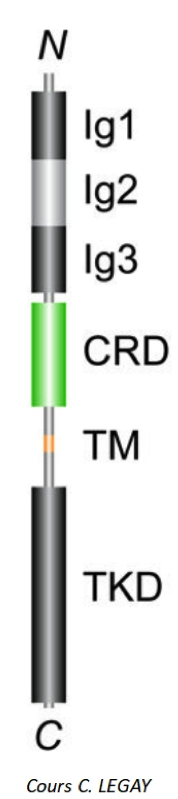
\includegraphics[width=0.1\textwidth]{./Images/MuSKReceptor.png}}
		\caption{Récepteur \gls{musk}}
		\descfig{Ig : Domaine immunoglobuline, CRD : \emph{Cysteine Rich Domain}, TM : Domaine transmembranaire,TKD : Domaine tyrosine kinase.}
		\label{fig:RMuSK}
	\end{wrapfigure}

	\gls{musk} est un récepteur découvert dans l'organe électrique de la raie \emph{Torpedo california} \cite{Jennings1993}. L'expression de ce récepteur à d'abord été mesurée dans les cellules musculaires et localisée au niveau de la \gls{jnm}. \gls{musk} est une récepteur tyrosine-kinase de 98kDa, dans lequel on distingue trois parties : un ectodomaine (partie N-terminale), un domaine transmembranaire, et un domaine cytoplasmique qui porte l'activité kinasique (voir \cref{fig:RMuSK}). 
	
	La partie extracellulaire comporte généralement trois domaines \gls{ig}, dont le domaine \gls{ig}1 a récemment été impliqué dans la liaison avec \gls{lrp}4 \cite{Zhang2011}, ainsi qu'un domaine Frizzled-like, riche en cystéines (\gls{crd}) \cite{Jing2009}.
	
	\gls{musk} possède trois ligand connu : l'Agrine (via \gls{lrp}4), un collagène spécifique associé à l'\Gls{ache} (\acrshort{colq} ), et les \Glspl{wnt}, tous nécessaire au développement complet de la synapse. Un défaut de signalisation de l'un d'entre eux entraîne ainsi des défauts structuraux et/ou fonctionnels de la synapse.
	
	La présence de \gls{musk} dans le cerveau a longtemps été ignorée, du fait de sa faible expression dans cette organe, quantifiée dans le passé par Northern Blot, une méthode de détection des \acrshort{arnm} trop peu sensible. Cependant, de nouvelles techniques, telle que l'\gls{his} ou bien la \gls{qpcr}, ont permis de montrer que le récepteur était bien présent dans le tissu cérébral, principalement au niveau des neurones du cortex, du cervelet, et de l'hippocampe \cite{Garcia-Osta2006, Ksiazek2007}. Le récepteur \gls{musk} est exprimé aussi dans les astrocytes \cite{Sun2016}, à des taux jusqu'à 5 fois supérieur à son expression dans les muscles squelettiques, où avec son co-récepteur \gls{lrp}4 il régulerait transmission glutamatergiques au travers du relargage d'ATP et une signalisation liée à l'agrine.
	
	Au niveau du \gls{snc}, deux isoformes de \gls{musk} semblent être exprimées \cite{Garcia-Osta2006}. La première isoforme, de 2644pbs, est identique à un épissage alternatif retrouvés dans le muscle \cite{Valenzuela1995}, sans qu'aucun rôle ne lui soit connu pour l'instant. La seconde isoforme est plus courte : 2359pbs, et présente une délétion du troisième domaine \gls{ig}. Les deux isoformes présentent une alanine à la position 454 qui remplace une délétion de 8a.a de l'éctodomaine. Une autre isoforme ayant le domaine \gls{ig}3 supprimé serait impliquée dans l'agrégation des \gls{achr} \cite{Hesser1999}.
	
	Grâce à des techniques de knockdown du gène par séquence antisens au niveau de l'hippocampe, il apparaîtrait que la présence de \gls{musk} dans le cerveau serait nécessaire mais non indispensable à la formation de la mémoire à moyen et long-terme \cite{Garcia-Osta2006}. La voie \gls{creb} est une voie impliquée dans la formation de la mémoire au niveau de l'hippocampe \cite{Silva1998, Kandel2012,Kida2014,Ortega-Martinez2015}, qui passerait par la phosphorylation de \gls{creb} suite au relargage de \acrshort{camp}, augmentant son activité transcriptionnelle. Un modèle propose \cite{Garcia-Osta2006} que l'activation de \gls{musk} activerait la cascade de signalisation de \gls{creb}, permettant la consolidation de la mémoire. Ce modèle expliquerait également l'auto-régulation de \gls{musk} \cite{Moore2001}, dont le gène possède dans sa séquence promotrice un élément CRE-like liant \gls{creb} \cite{Kim2005}. De plus, \gls{musk} est nécessaire à la formation de la \gls{ltp} de l'hippocampe \cite{Garcia-Osta2006}.
	
\section{Protéines \Acrshort{wnt}}
	\label{sec:IntroWnt}

	\begin{wrapfigure}{l}{0.4\textwidth}
		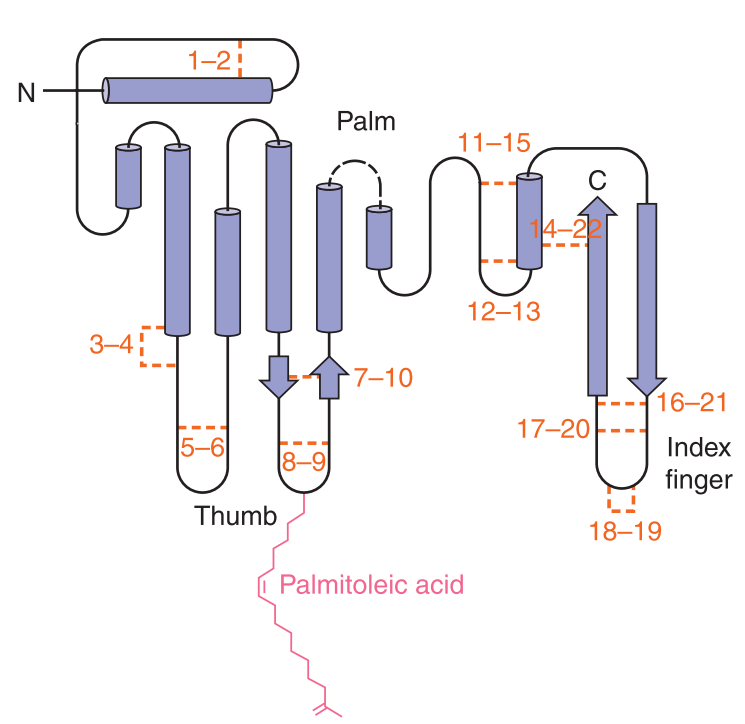
\includegraphics[width=0.4\textwidth]{./Images/WntProtein.png}	
		\caption{Structure d'une protéine \Gls{wnt} classique.}
		\descfig{Figure issue de Willert \& Nusse 2012 \cite{Willert2012}. En orange sont représentés les 22 résidus cystéines.}
		\label{fig:WntProt}
	\end{wrapfigure}
	
	Les protéines \gls{wnt} sont des glycoprotéines sécrétées, de 40kDa pour 350 acides aminés, impliquées dans de nombreux processus développementaux tel que l'embryogenèse, la prolifération, la différenciation, la migration cellulaire, ou encore l'apoptose \cite{Miller2002, Willert2012}. La structure des \Glspl{wnt} est complexe, avec  de nombreux ponts disulfures caractéristiques de cette famille de protéines, d'hélices \textalpha{}, ainsi que la présence d'un acide palmitoléïque participant à la liaison avec le récepteur (voir \cref{fig:WntProt}). On peut également souvent observé la présence d'un acide palmitique conservé au cours de l'évolution. La présence de ces acides gras rendent les protéines \Gls{wnt} très hydrophobes, ce qui a retardé leurs caractérisations.
	
	En plus de leurs rôles durant le développement, les \Glspl{wnt} jouent également un rôle à l'age adulte dans la maintenance des tissus adultes. Des travaux ont pu montré que les \Glspl{wnt} étaient également impliquées dans des étapes précoces de la formation de la \gls{jnm} \cite{Hall2000}. On connaît actuellement 19 membres de cette famille de protéine chez la souris et chez l'humain. Classiquement, les \Glspl{wnt} se lient sur le domaine \gls{crd} de leur récepteur \gls{fz}, associé aux co-récepteurs \gls{lrp}5 ou 6, mais il existe d'autres récepteurs non canoniques tels que : \gls{ror} \cite{Cadigan2006, Gordon2006, Green2008}, \gls{ryk} \cite{Bovolenta2006, Fradkin2010}, ou bien encore \gls{musk} \cite{Jing2009}, qui possèdent également un \gls{crd}.
	
	Il a été montré \emph{in vitro} que plusieurs \Glspl{wnt} interagissaient avec \gls{musk} : \Gls{wnt}2, 3a, 4, 6, 7b, 9a, et 11 \cite{Strochlic2012, Zhang2012, Barik2014}, avec différents effets. Seules \gls{wnt}4, 9a et 11 vont conduire à une dimérisation de \gls{musk} et a son activation (\emph{in vitro}). Ceci est cohérent avec le fait que chez le Poisson-zèbre, l'orthologue de \gls{musk}, \emph{unplugged}, le \gls{crd} allait interagir avec des protéines \Glspl{wnt} pour induire l'agrégation de \gls{achr} \cite{Jing2009, Gordon2012}. \Gls{lrp}4 semble être également nécessaire à l'agrégation des \gls{achr} médié par les \gls{wnt}s \cite{Zhang2012}.
	
	Les protéines \gls{wnt} peuvent activer plusieurs voies de signalisation différentes dans la cellule :  la voie canonique/\textbeta{}-catenin, la voie \gls{pcp}, et la voie \gls{wnt}/Calcium. Pour la voie canonique, en l'absence de \Glspl{wnt} sur le récepteur \gls{fz}, la \textbeta{}-catenin est continuellement reconnue par le complexe \acrshort{gsk3}-\acrshort{apc}-\acrshort{ck1}. Ce complexe va phosphorylé la \textbeta{}-catenin, permettant sa reconnaissance par la \gls{btrcp}, une E3 ubiquitine-ligase et son marquage pour destruction par le protéasome. Quand les \Glspl{wnt} se lient à \emph{\gls{fz}}, \emph{Dishevelled} (une protéine centrale dans les différentes voie \gls{wnt} \cite{Gao2010}) est recruté à la membrane, permettant l'interaction de \gls{lrp}5/6 avec \gls{gsk3}. Cette interaction va libéré la \textbeta{}-catenin qui s'accumule dans le cytoplasme, puis se translocalise dans le noyau, d'où elle va avoir un effet sur la transcription des gènes. 
	
	La voie \gls{pcp} est impliquée principalement dans la migration et la polarisation cellulaire. Les \Glspl{wnt} en se liant à \gls{fz} vont recrutés \emph{Dishevelled} 

	
\section{Contexte}
	\label{sec:Contexte}
	
	Dans le but d'étudier le rôle de l'interaction des protéines \Glspl{wnt} et du domaine \gls{crd} de \gls{musk}, l'équipe de C. LEGAY à crée une souris transgénique dont le \gls{crd} était supprimé (\mcrd) \cite{Messeant2015, Messeant2017}. Il a ainsi été montré que le \gls{crd} était nécessaire à la \gls{jnm} à la fois pour sa formation et pour son maintien à l'age adulte, et que \Gls{wnt}4 et 11 participaient activement à la formation de cette dernière. De plus, un traitement au \gls{licl} (inhibiteur de la \gls{gsk3}) permettait à la \gls{jnm} un retour vers un phénotype sauvage. 
	
	En plus de leurs problèmes musculaires, les souris \mcrd exhibaient des défauts centraux : durant son stage, une étudiante, Bertille SOMON, a montré que les mutants mâles avaient des blessures importantes au niveau du dos, blessures qui n'étaient pas dues à des comportements d'agressivité entre souris. De plus, une analyse comportementale a été réalisée en collaboration avec le groupe du Dr LANFUMEY (Centre de Psychiatrie et Neurosciences, Paris), et le test \gls{nor} a révélé que les souris mutantes souffraient d'une modification de la mémoire intermédiaire.
	
\section{But du stage}
\label{sec:IntroBut}

Comme \gls{musk} est exprimé dans le cerveau adulte, principalement au niveau de l'hippocampe \cite{Garcia-Osta2006}, et que ce lieu joue un rôle prépondérant dans la formation de la mémoire intermédiaire, l'objectif de mon stage va être d'explorer le rôle de l'interaction de \gls{musk} et des \Glspl{wnt} dans le cerveau, utilisant pour cela les souris \mcrd.

Cela se fera au travers de 5 axes : 
\begin{enumerate}
	\item Quelle est l'origine des blessures chez le mâle ?
	\item La structure du cerveau est-elle affectée chez le mutant ?
	\item Quelles sont les cellules exprimant \gls{musk} ?
	\item Quel est le niveau d'expression de \gls{musk}/\mcrd dans le cerveau ?
	\item Un traitement au \gls{licl} peut-il permettre un retour du mutant à un phénotype sauvage au niveau du comportement ?
\end{enumerate}